% Chapter 1

\chapter{Background} % Main chapter title

\label{back} % For referencing the chapter elsewhere, use \ref{Chapter1}

\lhead{Chapter 2. \emph{
Background}} % This is for the header on each page - perhaps a shortened title
The present work relied on two important concepts: gamification and spaced repetition. An overview of both concepts sets the stage for the proposed solution. Gamification provides an alternative to improve user experience, whereas spaced repetition offers a way to ease the retention of new knowledge. Among the several alternatives that implement spaced repetition, Anki and its mobile interface, AnkiDroid, provide a general purpose approach with a large user base. In addition, casual games offer characteristics that make them adaptable to non-leisure contexts including learning. One example is the 2048 game \citep{uberspot2017game} that has been subject of several studies. Finally, statistical testings allow to make inferences about the outcome of an experiment.

%----------------------------------------------------------------------------------------
\section{Gamification}
Gamification can be defined as the process of adding game elements and mechanics into non-game contexts \citep{deterding2011game}. The main objective of gamification is to improve the user experience and increase the motivation to use a product or service. To accomplish such an objective, gamification takes advantage of the inherent nature of humans to play. Unlike mandatory activities such as study and work, playing is voluntary and free; its main outcome is a feeling of joy and excitement \citep{johan1950homo}. These conditions set the environment for the adoption of game concepts and techniques in broader contexts.

Over the past ten years, gamification has attracted the attention of industry and academia. In the industry, companies have found a means to improve the performance and commitment of employees by avoiding traditional schemes of monetary rewards and punishments. Moreover, gamification provides a set of tools to increase the loyalty and engagement of users and customers. In the academia, gamification has expanded and merged various field of research given its interdisciplinary nature. It has attracted the attention of researchers in areas such as Human-Computer Interaction, Software Development, Psychology, Pedagogy, Bussiness Management and others.

%----------------------------------------------------------------------------------------
\section{Spaced Repetition}
Spaced repetition is a technique that facilitates the retention of new knowledge. It leverages the spacing effect phenomenon to help learners memorize specific contents \citep{hintzman1974theoretical}. This phenomenon allows learners to increase their capacity of retention by acquiring new knowledge in short recurrent sessions rather than in a single massive revision. In its basic form, spaced repetition sets increasing intervals of time between subsequent review sessions of previously learned material. This means that the more challenging the content the more frequently is reviewed by a learner. Then, the frequency of repetition is adjusted as the learner progresses.

Among the various existing techniques for memorization, spaced repetition stands out due to its simplicity and flexibility. The duration of each revision along with the interval time between consecutive sessions is defined by the learner. In addition, the learner assesses the easiness of the content under revision to determine the frequency of repetition. Finally, Spaced Repetition is a technique that can be used to learn new content from any field, but it is especially useful when the number of items to memorize is large. Such characteristics allow the implementation of this technique as a piece of software, making it available to a wider audience.

%----------------------------------------------------------------------------------------
\section{AnkiDroid}
Anki is a platform that implements a general purpose solution for spaced repetition. Thus, it can be used to learn and memorize content from any field. Its community has created an extensive base of content in a multitude of categories including languages, art, science, and trivia. It provides several interfaces including desktop applications for Linux, Mac, and Windows. In mobile environments, it provides applications for iOS and Android devices. The version for Android devices is known as AnkiDroid which code is publicly available under the GNU general public license.

AnkiDroid has well-defined logic and visual structures \citep{zamora2011ankidroid} that implement most of the features presented in the desktop applications including creation and editing of flashcards, visualization of statistics of use, and synchronization with the Anki system to save progress. Moreover, it has been designed to be compatible with the majority of Android versions. Therefore, the application is available for a wide range of devices which have helped to increase its popularity as an educational tool as seen in Figure \ref{fig:anki-evolution}.

In addtion, AnkiDroid has an large community of members that collaborate, support and promote the use and development of the application in web forums and groups. In regards to its development, the structure of the code allows modifications in the application that add or remove new features. The application can be modified to connect to external services, collect information of use, or include new elements. These characteristics have allowed that an extensive number of contributors (131) be part of its development.

\begin{figure}[htb]
    \vskip 5mm
        \begin{center}
            \includegraphics[scale=0.4]{./Figures/anki_progress.png}
            \caption{Evolution of the number of installations of AnkiDroid. Image taken from the twitter account of AnkiDroid (https://twitter.com/AnkiDroid)}
            \label{fig:anki-evolution}
        \end{center}
    \vskip -5mm
\end{figure}


%----------------------------------------------------------------------------------------
\section{Casual Video Games}
A casual game has to be fun, it needs to provide a quick way to access, and the gameplay must be easy to understand, as defined by the Casual Games Association (CGA). These characteristics mean that users do not require any previous expertise or skills related to video games. For these reasons, casual games have a broad audience that includes people from all age groups.

The characteristics of this type of games have been leverage to adapt them to non-leisure contexts including health and learning. In the health context, the use of casual games has been studied as an alternative element to improve mood and decrease stress \citep{russoniello2009effectiveness}. Additional studies have demonstrated the effectiveness of playing casual games as a recovery strategy after periods of high work strain \citep{reinecke2009games}. Finally, casual games have also been studied as an alternative to traditional educational tools \citep{peirce2010personalised}

%----------------------------------------------------------------------------------------
\section{2048 Game}
2048 is a puzzle-like casual game cotaining a 4x4 grid as seen in Figure \ref{fig:2048-grid}. The objective of the game is to merge numbered blocks until creating one with the value 2048. The game starts with two blocks of value 2 which are randomly positioned in the grid. The player has to slide the blocks horizontally or vertically. The blocks move in the chosen direction; a block stops if it reaches an edge of the grid or collides with another block. If two colliding blocks have the same number, they are merged into a single block which value is the sum of the values of the forming blocks. In every turn, a new block of value 2 is randomly positioned in the grid.

\begin{figure}[htb]
    \vskip 5mm
        \begin{center}
            \includegraphics[scale=0.5]{./Figures/game_grid.png}
            \caption{Grid of the 2048 game.}
            \label{fig:2048-grid}
        \end{center}
    \vskip -5mm
\end{figure}

The popularity of the game has turned it into a subject of different types of studies. The majority of these studies aim to analyse the game from the computational complexity perspective \citep{abdelkader20162048}, and propose several artificial intelligence alternatives to win the game including neural networks \citep{boris2016evolving} and Monte-Carlo methods \citep{rodgers2014investigation}. However, the game has also been studied as an educational element to engage student interest \citep{neller2015pedagogical}

%----------------------------------------------------------------------------------------
\section{Statistical testing}
\label{stat-testing}
Statistical testing provides a way to make inferences about the data and tell if the observed pattern is real or due to chance. In research, this type of analysis helps to determine the effects of a treatment on the outcome and the robustness of that relationship. In comparative studies, a new treatment is applied to units in the experimental group, whereas units in the control group receive the standard treatment or not treatment at all.

The outcomes from the control and experimental groups can be described and compared by their means. The difference between both means gives some insights about the groups. However, the difference of means needs to be complimented with the variances of the samples to determine if it is statistically significant. This analysis can be done using the Student's t-test.

The Student's t-test is a method that can be used to do a statistical hyphotesis testing. The method provides a parameter called t-value that is the ratio bewteen a signal (difference of means) and noise (variability of samples). This parameter and the degrees of freedom (number of values that are free to vary) are used to find the probability value of having the same mean difference in additional experiments. Therefore, the probability value is used to confirm or deny the null hypothesis.

% % Add to description of game
%  the state of the grid is defined by the positions of the blocks and their values at a given turn
